\graphicspath{{\currfiledir/images/}}

\chapter{Conceitos Introdutórios}

%=====================================================

Este capítulo introduz brevemente os conceitos básicos de grafos que serão utilizados ao longo dessa dissertação. Os conceitos apresentados neste capítulo podem ser acessados nas seguintes bibliografias: \cite{bondymurty1976}; \cite{west2002}; \cite{bondymurty2008}; \cite{feofiloff2018}.


\section{Teoria de grafos}
Muitas situações do mundo real podem ser convenientemente descritas por meio de um diagrama que consiste em um conjunto de pontos, juntamente com linhas que unem certos pares desses pontos \cite{bondymurty1976}. Por exemplo, os pontos podem representar pessoas, com linhas unindo pares de amigos ou os pontos podem ser centros de comunicação, com linhas representando links de comunicação. Tais diagramas buscam saber se dois pontos dados são unidos por uma linha, a maneira pela qual eles são unidos é irrelevante. Uma abstração matemática de situações desse tipo dá origem ao conceito de grafos \cite{bondymurty2008}.

\begin{definition}
    Um grafo $G$ é denotado por um par ordenado $(V(G), E(G))$, onde $V(G)$ é um conjunto de vértices e $E(G)$ é um conjunto de ligações entre pares de vértices de $G$, chamados de arestas. São denotadas por $n = |V(G)|$ e $m = |E(G)|$ as cardinalidades dos conjuntos $V(G)$ e $E(G)$, respectivamente.
\end{definition}


\section{Direcionamento de grafos}
Usando-se das definições anteriores, nesta seção iremos explanar umas das principais propriedades da conectividade de grafos, seu direcionamento.

Considere a Figura~\ref{sec2:ex-grafo-nao-direcionado}. Este é um exemplos de um grafo $G$, não direcionado, onde $V(G) = {a, b, c, d}$ e $E(G) = {{a, b}, {a, c}, {a, d}, {b, c}, {b, d}, {c, d}}$. Nota-se que as arestas ${a, b}$ e ${b, a}$ são considerados redundantes, motivo pela qual o conjunto $E(G)$ apresenta somente uma delas.

\begin{figure}[!htb]
    \centering
    % 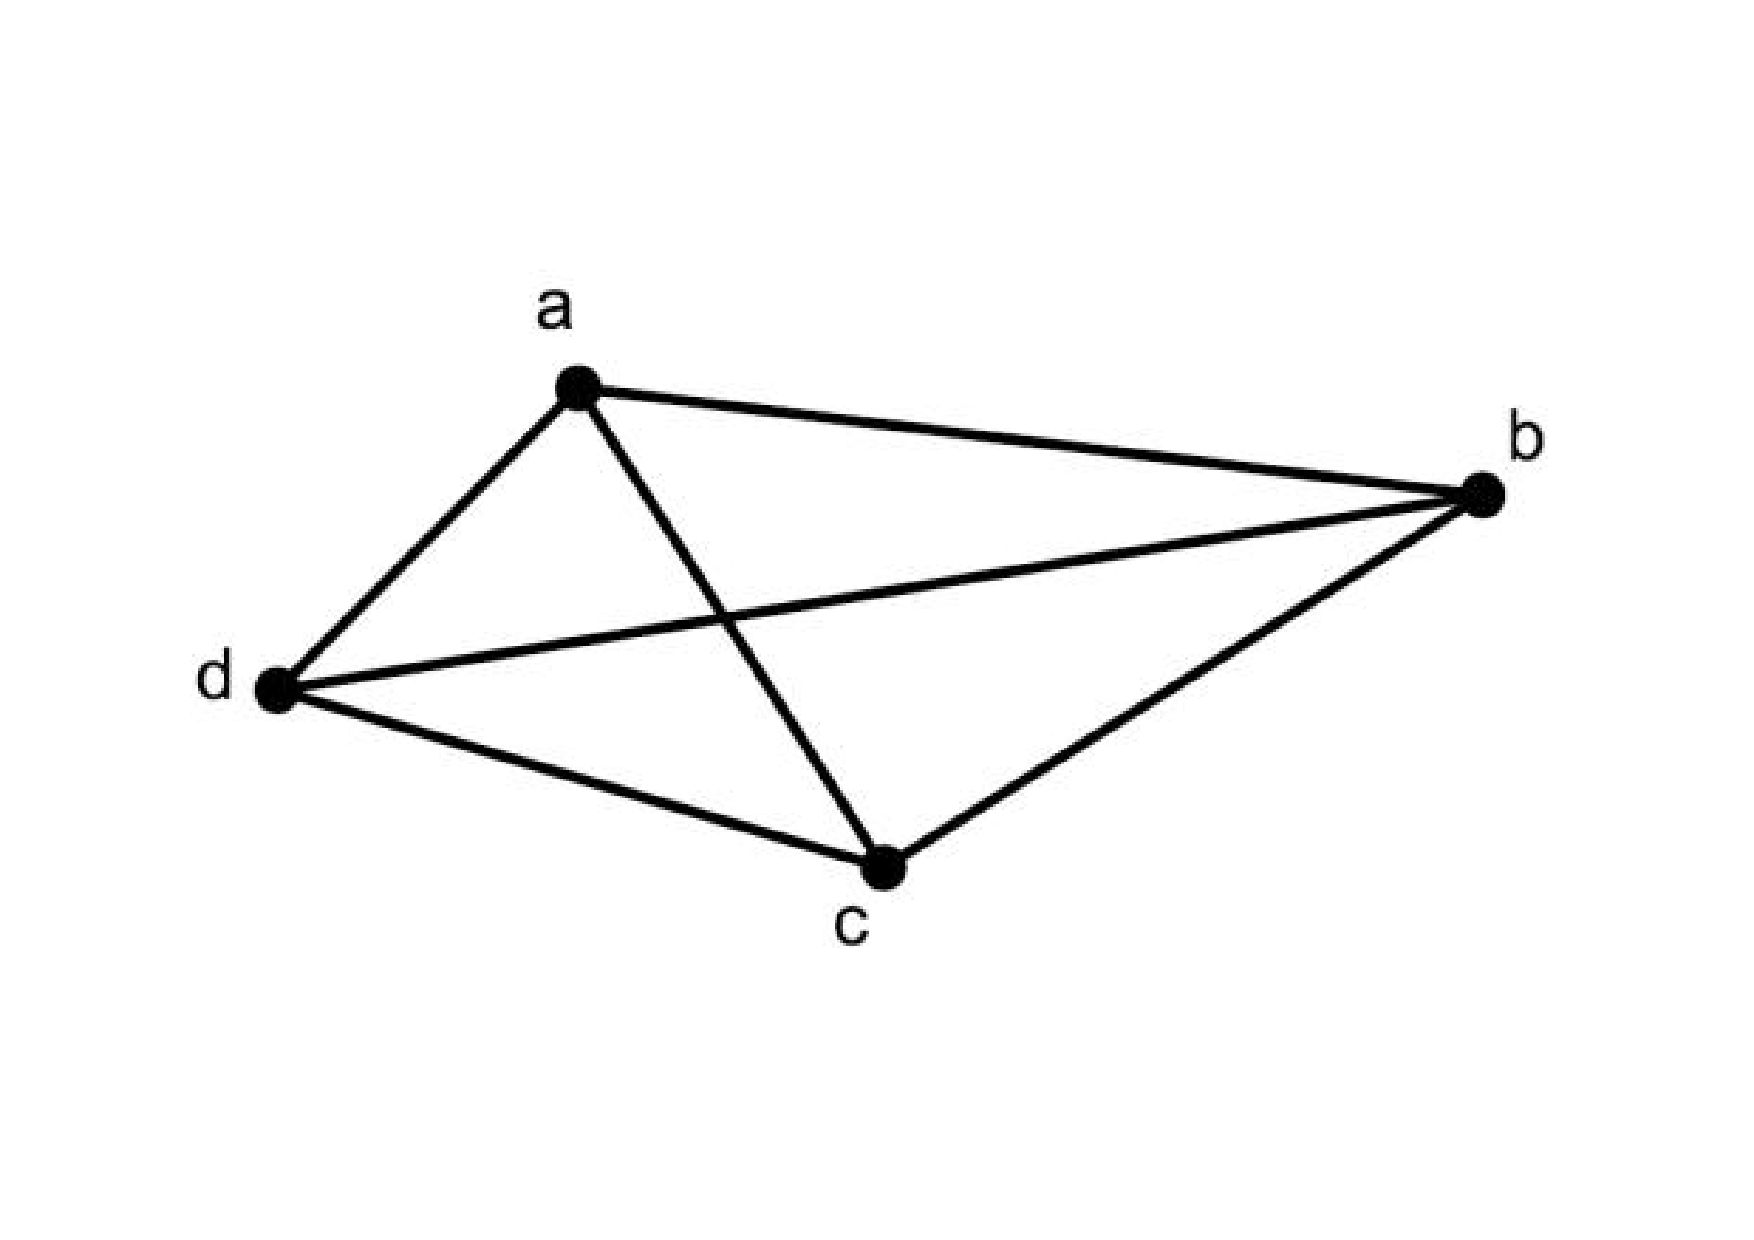
\includegraphics[width=\textwidth,height=\textheight,keepaspectratio]{grafo-nao-direcionado.pdf}
    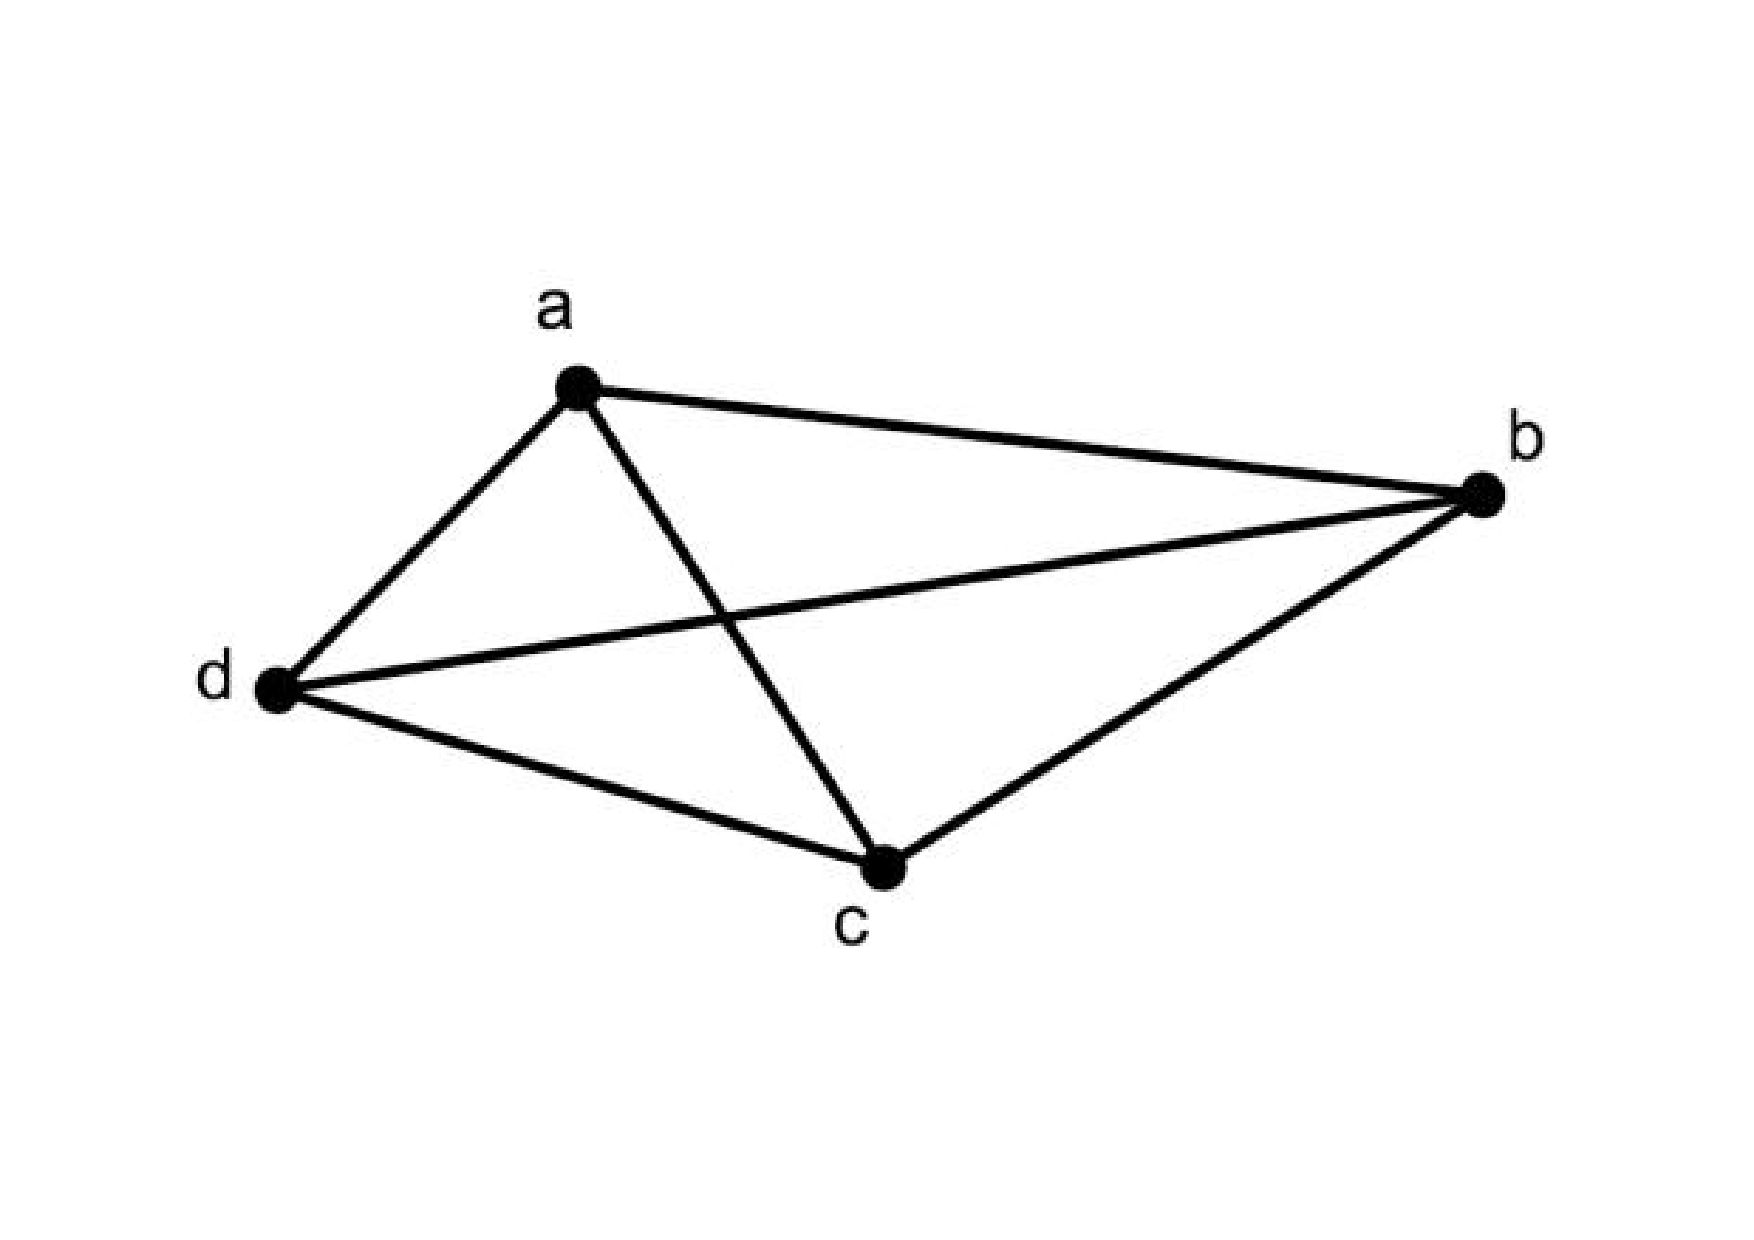
\includegraphics[scale=0.3]{grafo-nao-direcionado.pdf}
    \caption{Grafo não direcionado}
    \label{sec2:ex-grafo-nao-direcionado}
\end{figure}

Considere a Figura~\ref{sec2:ex-grafo-direcionado}. Este é um exemplos de um grafo $G$, direcionado, onde $V(G) = {a, b, c, d}$ e $E(G) = {ab, ad, bc, ca, db}$. A aresta $ab$, indica que há uma relação de $a$ para $b$ e esta relação não é comutativa, isto é, para este grafo $G$, a relação $ba$ não é verdade.

\begin{figure}
    \centering
    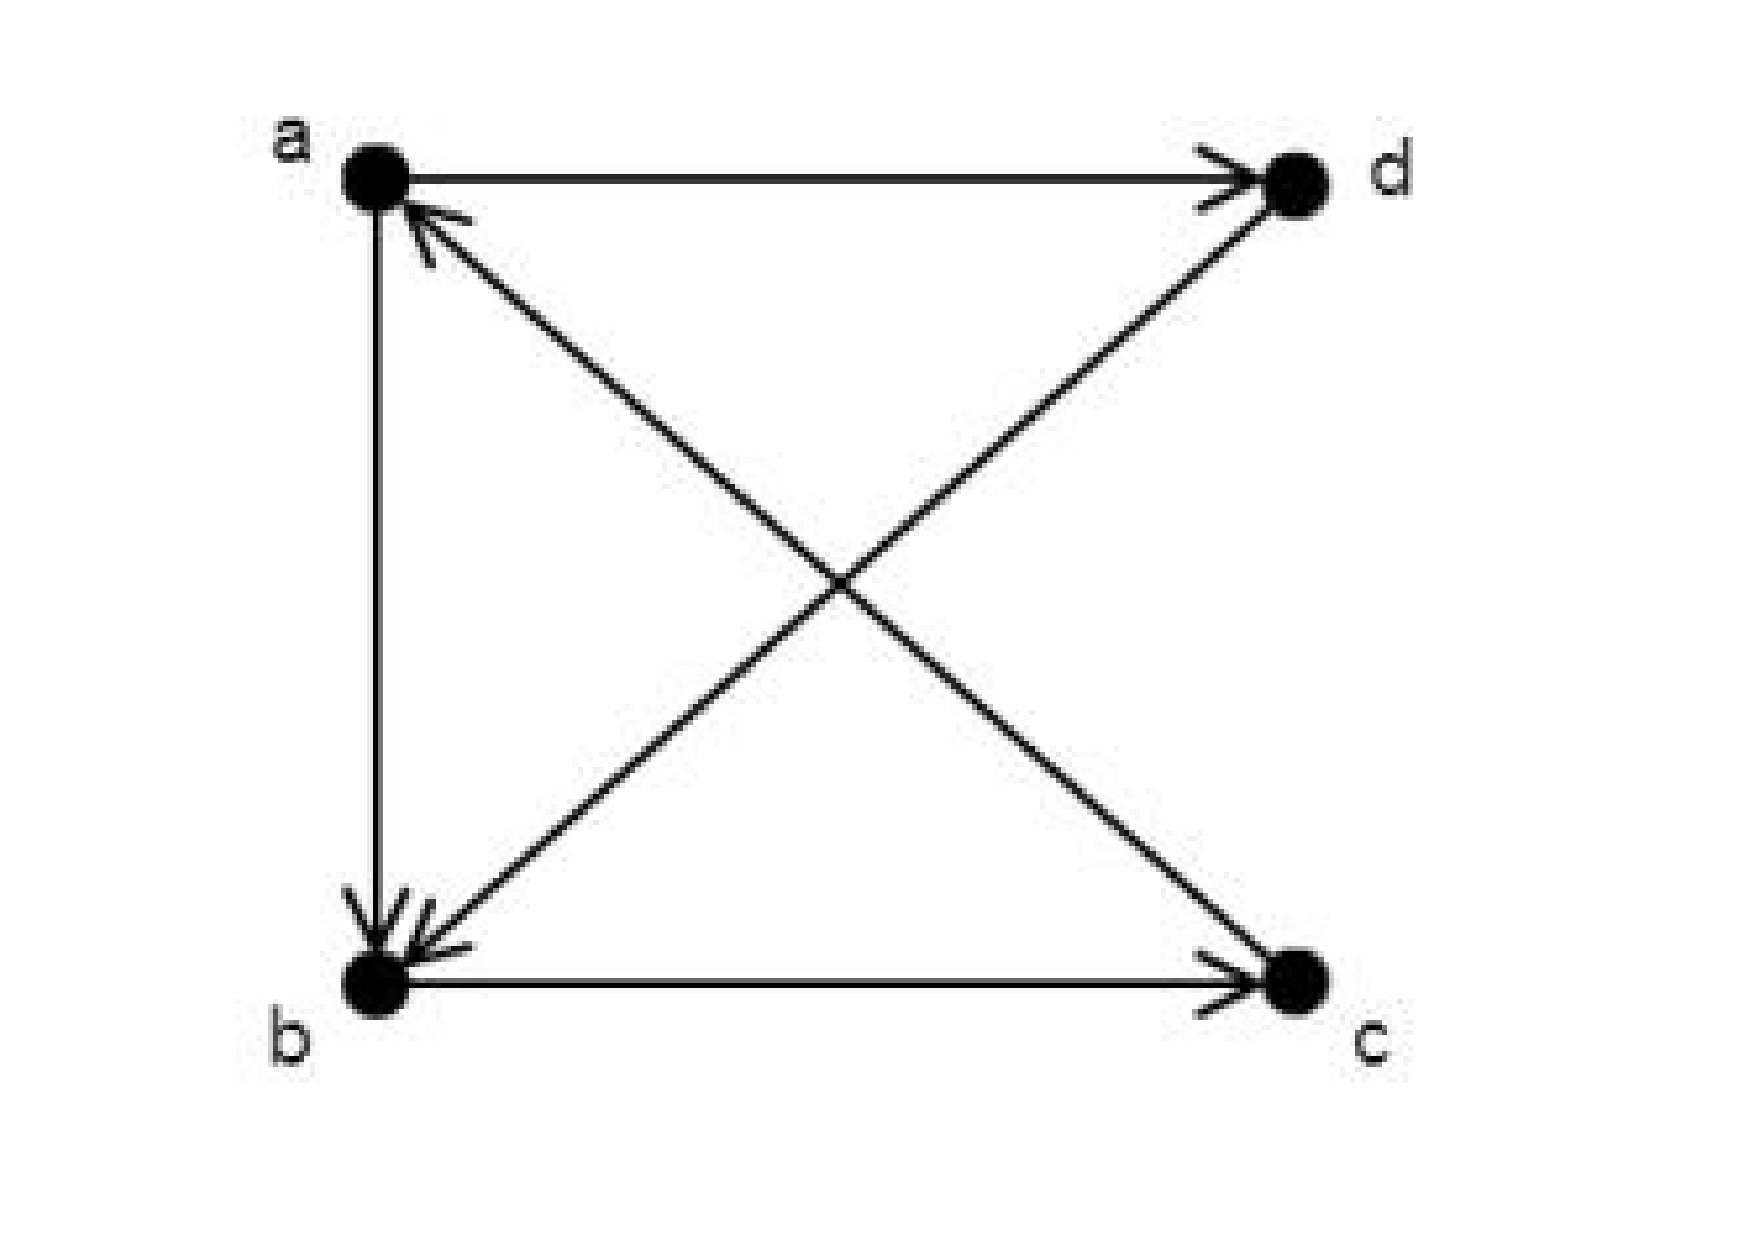
\includegraphics[scale=0.3]{grafo-direcionado.pdf}
    \caption{Grafo direcionado}
    \label{sec2:ex-grafo-direcionado}
\end{figure}




\section{Tipos de grafos}

% A introdução geral do documento pode ser apresentada através das seguintes seções: Desafio, Motivação, Proposta, Contribuição e Organização do documento (especificando o que será tratado em cada um dos capítulos). O Capítulo 1 não contém subseções\footnote{Ver o Capítulo \ref{cap-exemplos} para comentários e exemplos de subseções.}.

Este modelo foi proposto com o intuito de padronizar e simplificar as monografias, dissertações e teses produzidas no Departamento de Informática da UFPR. Ele foi vagamente inspirado nas normas da ABNT (conforme indicado em \cite{bibufpr15}), mas não as segue \emph{ipsis litteris}. Várias alterações foram feitas com o objetivo de melhorar sua estética e tornar o texto mais legível para trabalhos na área de informática. A versão atualizada deste modelo está disponível em \cite{maziero15}.

Este modelo está baseado em uma classe especifica \verb#ppginf.cls#, que aceita várias opções de compilação. A versão do documento pode ser:

\begin{itemize}

\item \verb#defesa#: é gerado um documento em espaço 1,5, frente simples e sem as páginas iniciais adicionais; é uma versão adequada para receber as anotações dos membros da banca de defesa.

\item \verb#final#: é gerado um documento em espaço simples, frente/verso, com páginas iniciais (capa, ficha catalográfica, folha de aprovação, agradecimentos, etc). É uma versão bem mais compacta, mais ecológica e ideal para a impressão definitiva.

\end{itemize}

Para obter os melhores resultados, compile este modelo usando a seguinte sequência de passos:

\begin{quote}
\begin{footnotesize}
\begin{verbatim}
pdflatex  main          // compilação inicial
bibtex main             // processa referências bibliográficas
pdflatex  main          // compilação final
\end{verbatim}
\end{footnotesize}
\end{quote}

ou

\begin{quote}
\begin{footnotesize}
\begin{verbatim}
make                    // faz tudo...
\end{verbatim}
\end{footnotesize}
\end{quote}

Os principais itens considerados na formatação deste documento foram:

\begin{itemize}

\item Papel em formato A4, com margens de 20 mm à direita e embaixo, 30 mm nos demais lados. Não devem ser usados cabeçalhos ou rodapés além dos que estão aqui propostos.

\item O texto principal do documento escrito em 12 pontos. O fonte principal do texto pode ser selecionado no arquivo \verb#packages.tex#.

\item Código-fonte, listagens e textos similares são formatados em fonte Courier 12 ou 10 pontos.

\item O espaçamento padrão entre linhas é 1,5 linhas (1 linha na versão final). Não inserir espaços adicionais entre parágrafos normais. Figuras, tabelas, listagens e listas de itens devem ter um espaço adicional antes e após os mesmos.

\item As páginas iniciais não são numeradas.

\item O corpo do texto é numerado com algarismos arábicos (1, 2, 3, ...) a partir da introdução, ate o final do documento. Os números de página devem estar situados no alto à direita (páginas direitas) ou à esquerda (páginas esquerdas).

\item Expressões em inglês, grego, latim ou outras línguas devem ser enfatizadas em itálico, como \emph{sui generis} ou \emph{scheduling} (use o comando \verb#\emph{...}#).

\item Para reforçar algo, deve-se usar somente \textbf{negrito}. \underline{Sublinhado} ou MAIÚSCULAS não devem ser usados como forma de ênfase!

\item As notas de rodapé também têm um modelo\footnote{As notas de rodapé dever ser escritas em tamanho 10 pt, numeradas em arábico.}. Notas de rodapé servem para fazer algum comentário paralelo; não as use para colocar URLs, referências bibliográficas ou significado de siglas.

\end{itemize}

Felizmente o \LaTeX\ resolve a maior parte dessas questões!

%=====================================================
